%
% teil3.tex -- Beispiel-File für Teil 3
%
% (c) 2020 Prof Dr Andreas Müller, Hochschule Rapperswil
%
\section{Beispiel Verfolgungskurve
\label{lambertw:section:teil4}}
\rhead{Beispiel Verfolgungskurve}
In diesem Abschnitt wird rechnerisch das Beispiel einer Verfolgungskurve beschreiben.

\subsection{Ziel bewegt sich auf einer Gerade
\label{lambertw:subsection:malorum}}
Das zu verfolgende Ziel \(\overrightarrow{Z}\) wandert auf einer Gerade, wobei diese Gerade der \(y\)-Achse entspricht. Der Verfolger \(\overrightarrow{V}\) startet auf einem beliebigen Punkt auf dem ersten Quadrant. Um die Rechnungen zu vereinfachen wir die Geschwindigkeit \(v\) auf 1 gesetzt. Diese Anfangspunkte oder Anfangsbedingungen können wie folgt formuliert werden:
\begin{equation}
	\overrightarrow{Z}
	=
	\left( \begin{array}{c} 0 \\ v \cdot t \end{array} \right)
	=
	\left( \begin{array}{c} 0 \\ t \end{array} \right)
	;
	\overrightarrow{V}
	=
	\left( \begin{array}{c} x \\ y \end{array} \right)
	\label{lambertw:Anfangspunkte}
\end{equation}
Wenn man diese Startpunkte in die Gleichung der Verfolgungskurve einfügt ergibt sich folgender Ausdruck:
\begin{equation}
	\frac{\left( \begin{array}{c} 0-x \\ t-y \end{array} \right)}{\sqrt{x^2 + (t-y)^2}}
	\circ
	\left(\begin{array}{c} \dot{x} \\ \dot{y} \end{array}\right)
	=
	1
	\label{lambertw:eqMitAnfangspunkte}
\end{equation}
Macht man den linken Term Bruchfrei und löst das Skalarprodukt auf, dann ergibt sich folgende DGL:
\[
	\left( \begin{array}{c} 0-x \\ t-y \end{array} \right)
	\circ
	\left(\begin{array}{c} \dot{x} \\ \dot{y} \end{array}\right)
	= \sqrt{x^2 + (t-y)^2}\\
\]
\begin{equation}
		-x \cdot \dot{x} + (t-y) \cdot \dot{y}
		= \sqrt{x^2 + (t-y)^2}
		\label{lambertw:eq1BspVerfolgKurve}
\end{equation}
Im nächsten Schritt quadriert man beide Seiten, erweitert den neu entstandenen quadratischen Term, bringt alles auf die linke Seite und klammert gemeinsames aus.
\begin{align*}
	((t-y) \dot{y} - x \dot{x})^2
	&= x^2 + (t-y)^2 \\
	x^2 \dot{x}^2 - 2x(t-y) \dot{x} \dot{y} + (t-y)^2 \dot{y}
	&= x^2 + (t-y)^2 \\
	\dot{x}^2 x^2 - x^2 - 2x(t-y) \dot{x} \dot{y} + \dot{y}^2 (t-y)^2 - (t-y)^2
	&= 0 \\
	(\dot{x}^2 - 1) \cdot x^2 - 2x(t-y) \dot{x} \dot{y} + (\dot{y}^2 - 1) \cdot (t-y)^2
	&= 0
\end{align*}
Der letzte Ausdruck kann mittels folgender Beziehung \(\dot{x}^2 + \dot{y}^2 = 1\) vereinfacht werden, anschliessend wird die Gleichung mit \(-1\) multipliziert:
\[
	\underbrace{(\dot{x}^2 - 1)}_{\mathclap{-\dot{y}^2}} \cdot x^2 - 2x(t-y) \dot{x} \dot{y} + \underbrace{(\dot{y}^2 - 1)}_{\mathclap{-\dot{x}^2}} \cdot (t-y)^2
	= 0
\]
\begin{align*}
	- \dot{y}^2 \cdot x^2 - 2x(t-y) \dot{x} \dot{y} - \dot{x}^2 \cdot (t-y)^2
	&= 0 \\
	\dot{y}^2 \cdot x^2 + 2x(t-y) \dot{x} \dot{y} + \dot{x}^2 \cdot (t-y)^2
	&= 0
\end{align*}
Im letzten Ausdruck erkennt man das Muster einer binomischen Formel, was den Ausdruck wesentlich vereinfacht:
\begin{align*}
	x^2 \dot{y}^2  + 2 \cdot x \dot{y} \cdot (t-y) \dot{x}  + (t-y)^2 \dot{x}^2
	&= 0 \\
	(x \dot{y} + (t-y) \dot{x})^2
	&= 0
\end{align*}
Wenn man nun beidseitig die Quadratwurzel zieht, dann ergibt sich im Vergleich zu \eqref{lambertw:eq1BspVerfolgKurve} eine wesentlich einfachere DGL:
\begin{equation}
	x \dot{y} + (t-y) \dot{x}
	= 0
	\label{lambertw:equation5}
\end{equation}
Um die Ableitung nach der Zeit wegzubringen, wird beidseitig mit \(\dot{x}\) dividiert, wobei \(\frac{\dot{y}}{\dot{x}} = \frac{dy}{dt}/\frac{dx}{dt} = \frac{dy}{dx}\) entspricht.
\[
	x \frac{\dot{y}}{\dot{x}} + (t-y) \frac{\dot{x}}{\dot{x}}
	= 0
\]
Nach dem Kürzen und Vereinfachen ergibt sich folgende DGL:
\begin{equation}
	x y^{\prime} + t - y
	= 0
	\label{lambertw:DGLmitT}
\end{equation}
Hier wäre es passend wenn man die Abhängigkeit nach \(t\) komplett wegbringen könnte. Um dies zu erreichen muss man auf die Definition der Bogenlänge aus Analysis 2 zurückgreifen:
\begin{equation}
	s
	= 
	v \cdot t
	=
	t
	=
	\int_{x_0}^{x_{end}}\sqrt{1+y^{\prime\, 2}} \: dx
	\label{lambertw:eqZuBogenlaenge}
\end{equation}
Nicht gerade auffällig ist die Richtung in welche hier integriert wird. Wenn der Verfolger sich wie vorgesehen am Anfang im ersten Quadranten befindet, dann muss sich dieser nach links bewegen, was nicht der üblichen Integrationsrichtung entspricht. Um eine Integration wie üblich von links nach rechts ausführen zu können, müssen die Integrationsgenerzen vertauscht werden, was in einem Vorzeichenwechsel resultiert. Wenn man nun \eqref{lambertw:eqZuBogenlaenge} in die DGL \eqref{lambertw:DGLmitT} einfügt, dann ergibt sich folgender Ausdruck:
\begin{equation}
	x y^{\prime} - \int\sqrt{1+y^{\prime\, 2}} \: dx - y
	= 0
	\label{lambertw:DGLohneT}
\end{equation}
Um das Integral los zu werden, leitet man den vorherigen Ausdruck \eqref{lambertw:DGLohneT} nach \(x\) ab:
\begin{align*}
	y^{\prime}+ xy^{\prime\prime} - \sqrt{1+y^{\prime\, 2}} - y^{\prime}
	&= 0 \\
	xy^{\prime\prime} - \sqrt{1+y^{\prime\, 2}}
	&= 0
\end{align*}
Mittels der Substitution \(y^{\prime} = u\) kann vorherige DGL in eine erster Ordnung umgewandelt werden:
\begin{equation*}
	xu^{\prime} - \sqrt{1+u^2}
	= 0
	\label{lambertw:DGLmitU}
\end{equation*}
Welche mittels Separation gelöst werden kann:
\begin{align*}
	arsinh(u) + C_L
	&=
	ln(x) + C_R \\
	arsinh(u)
	&=
	ln(x) + C \\
	u
	&=
	sinh(ln(x) + C)
\end{align*}
In dem man die Substitution rückgängig macht, erhält man eine weitere DGL erster Ordnung die bereits separiert ist:
\begin{equation}
	y^{\prime}
	=
	sinh(ln(x) + C)
\end{equation}
Diese kann mit den selben Methoden gelöst werden, diesmal in Kombination mit der exponentiellen Definition der \(sinh\)-Funktion:
\begin{align*}
	y
	&=
	\int sinh(ln(x) + C) \\
	&=
	\int \frac{1}{2} (e^{ln(x)+C} - e^{-(ln(x)+C)}) \\
	&=
	\frac{e^C}{4} x^2 - \frac{ln(x)}{2 \cdot e^C} + C_1 \\
	&=
	C_1 + C_2 x^2 - \frac{ln(x)}{8 \cdot C_2}
\end{align*}

\begin{figure}
	\centering
	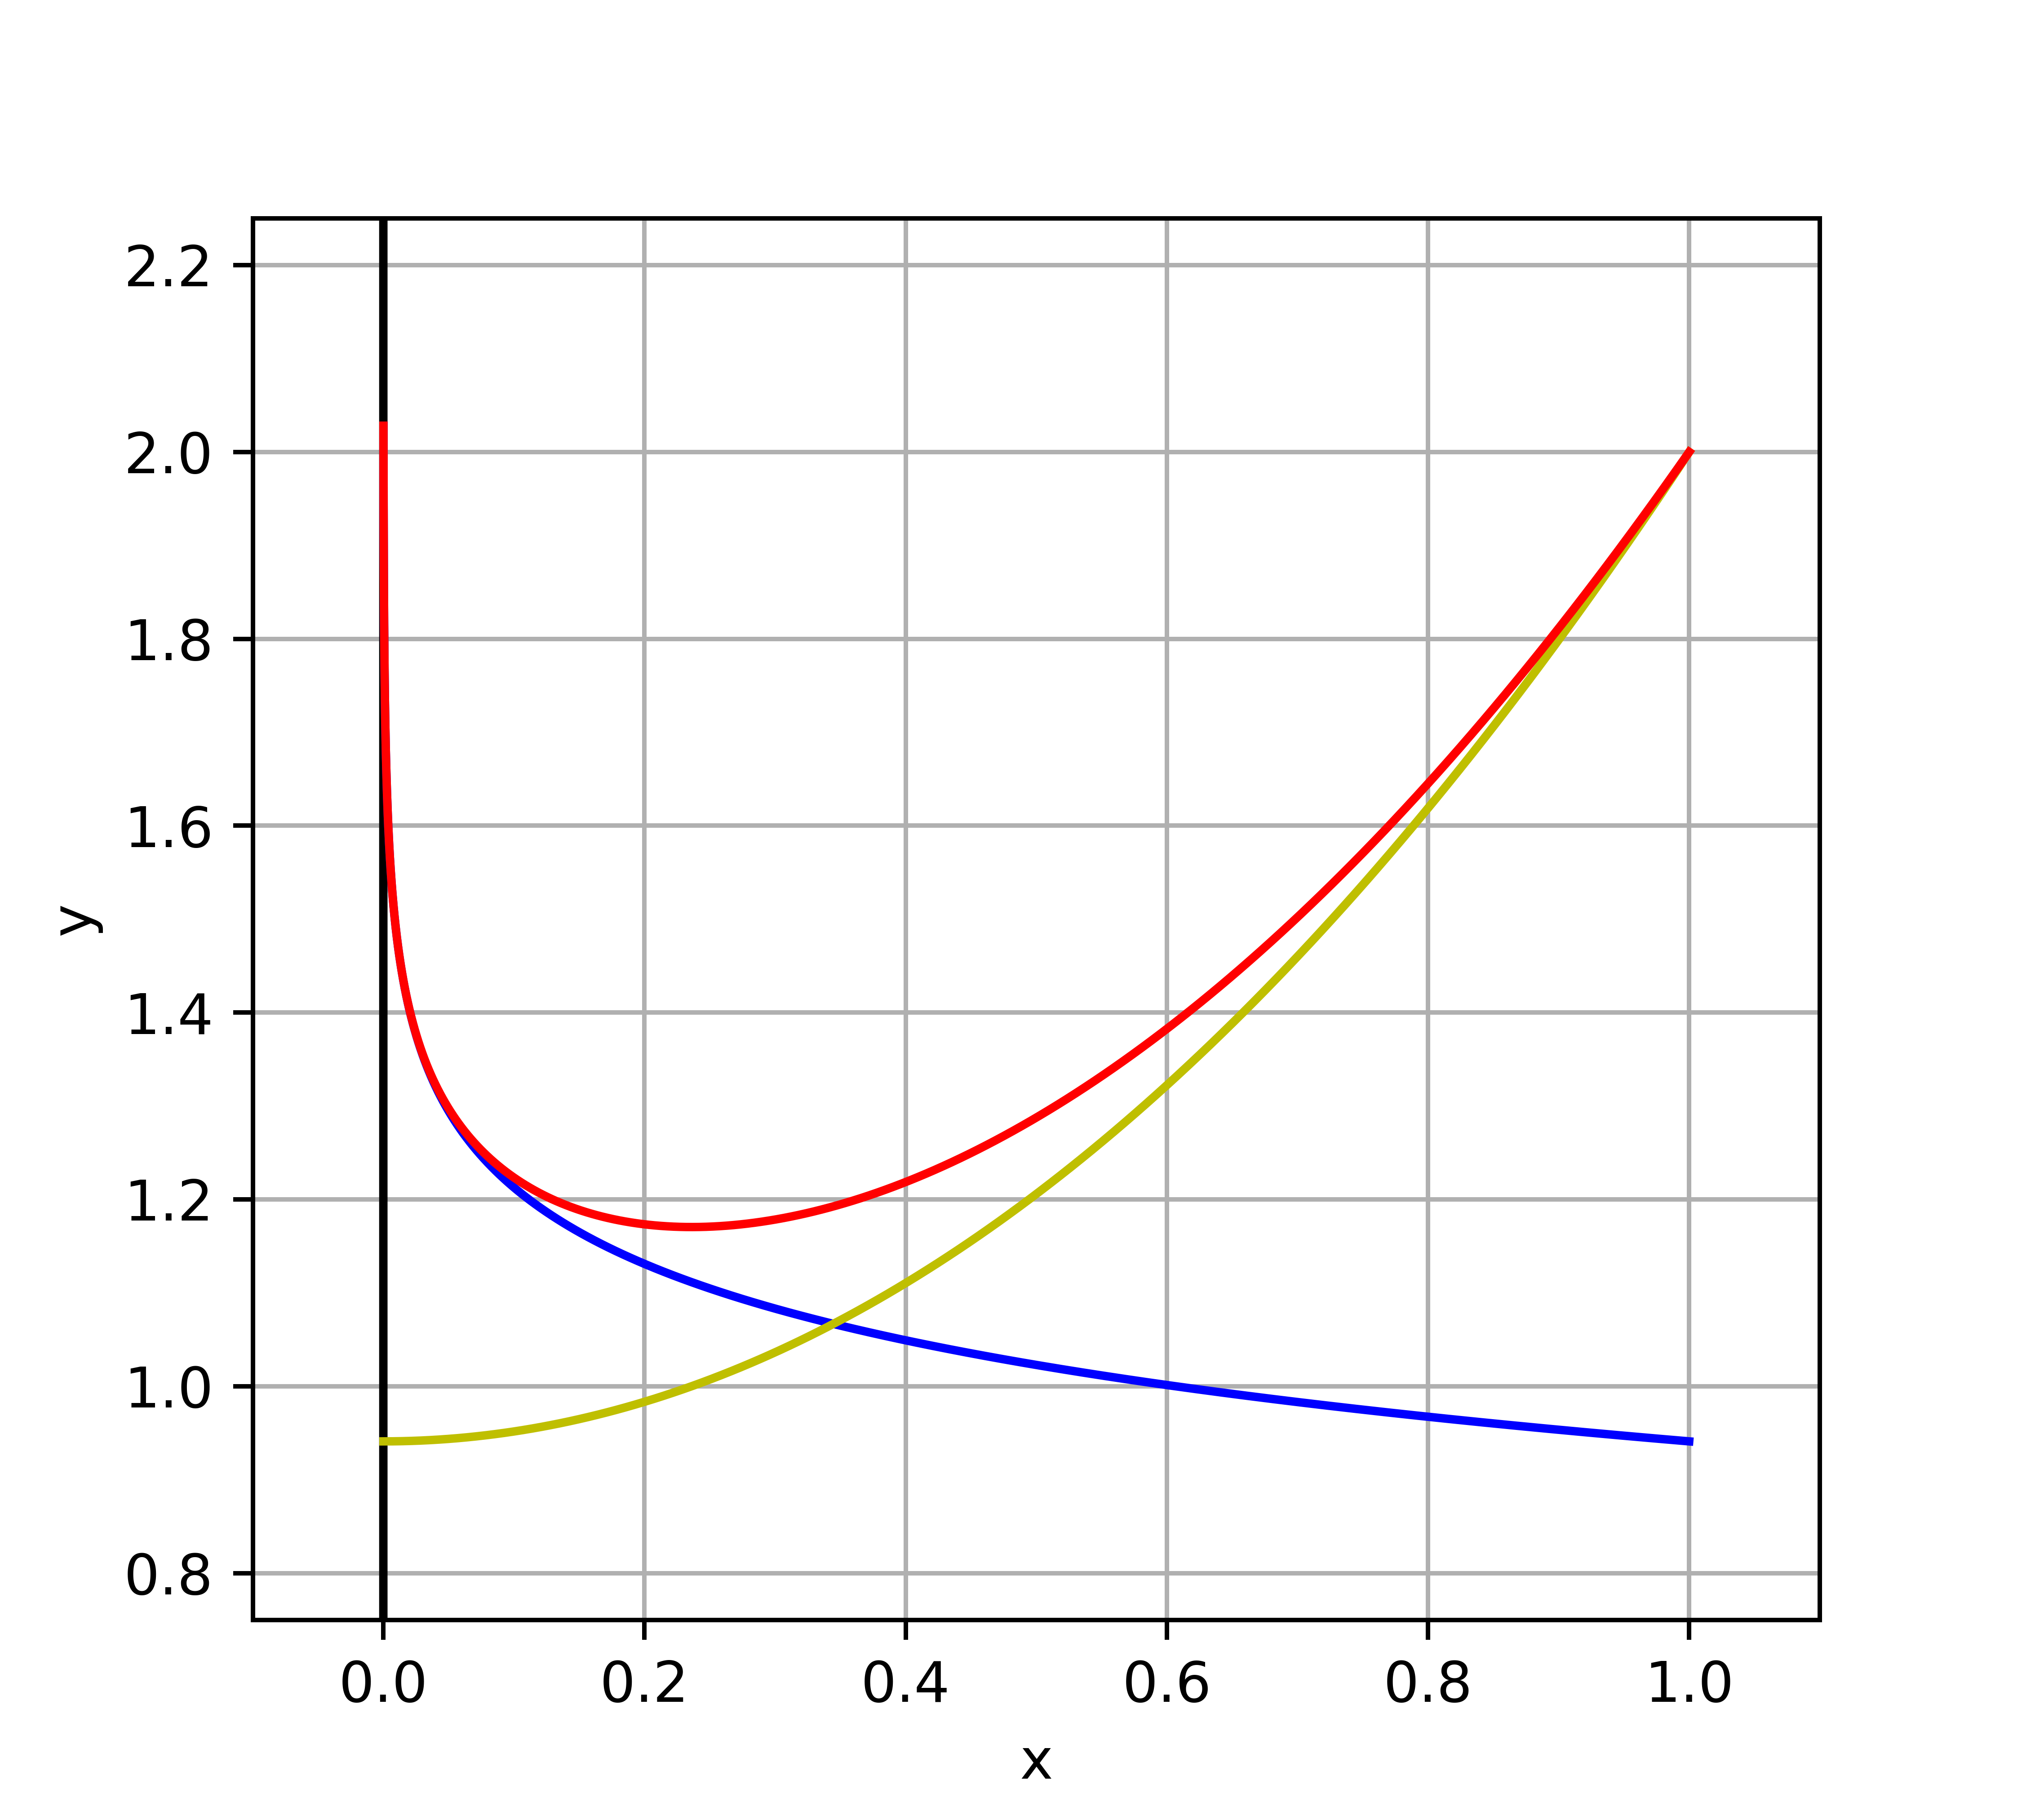
\includegraphics{papers/lambertw/Bilder/VerfolgungskurveBsp.png}
	\caption[Graph der Verfolgungskurve]{Graph der Verfolgungskurve wobei, ({\color{red}rot}) die Funktion \ensuremath{y(x)} ist, ({\color{darkgreen}grün}) der quadratische Teil und ({\color{blue}blau}) dem \ensuremath{ln(x)}-Teil entspricht.
	\label{lambertw:funkLoes}
	}
\end{figure}

Das Resultat, wie ersichtlich, ist folgende Funktion \eqref{lambertw:funkLoes} welche mittels Anfangsbedingungen parametrisiert werden kann: 
\begin{equation}
	{\color{red}{y(x)}}
	=
	C_1 + C_2 {\color{darkgreen}{x^2}} {\color{blue}{-}} \frac{\color{blue}{ln(x)}}{8 \cdot C_2}
	\label{lambertw:funkLoes}
\end{equation}
Für die Koeffizienten \(C_1\) und \(C_2\) ergibt sich ein Anfangswertproblem, welches für deren Bestimmung gelöst werden muss. Zuerst soll aber eine qualitative Intuition, oder Idee für das Aussehen der Funktion \(\bf{y(x)}\) geschaffen werden:
\begin{itemize}
	\item
	Für grosse \(x\)-Werte welche in der Regel in der Nähe von \(x_0\) sein sollten, ist der quadratisch Term in der Funktion dominant und somit für immer kleiner werdende \(x\) geht der Verfolger in Richtung \(y\)-Achse wobei seine Steigung stetig sinkt, was Sinn macht wenn der Verfolgte entlang der \(y\)-Achse steigt.
	\item
	Für \(x\)-Werte in der Nähe von \(0\) ist das asymptotische Verhalten des Logarithmus dominant, dies macht auch Sinn da sich der Verfolgte auf der \(y\)-Achse bewegt und der Verfolger im nachgeht.
	\item
	Aufgrund des Monotoniewechsels in der Kurve muss es auch ein Minimum aufweisen. Es stellt sich nun die Frage: Wo befindet sich dieser Punkt? Durch eine logische Überlegung kann eine Abschätzung darüber getroffen werden und zwar, dass dieser dann entsteht, wenn \(A\) und \(P\) die gleiche \(y\)-Koordinaten besitzen. In diesem Moment ändert die Richtung der \(y\)-Komponente der Geschwindigkeit und somit auch sein Vorzeichen.
\end{itemize}
Alle diese Eigenschafte stimmen mit dem überein, was man von einer Kurve dieser Art erwarten würde. Nun stellt sich die Frage wie die Kurve wirklich aussieht, dies wird durch das Einsetzen folgender Anfangsbedingungen erreicht:
\begin{equation}
	y(x)\big \vert_{t=0}
	=
	y(x_0)
	= 
	y_0
	\:;\:
	\frac{dy}{dx}\bigg \vert_{t=0}
	=
	y^{\prime}(x_0)
	=
	\frac{y_0}{x_0}
\end{equation}
Leitet man die Funktion \eqref{lambertw:funkLoes} nach x ab und setzt die Anfangsbedingungen ein, dann ergibt sich folgendes Gleichungssystem:
\begin{subequations}
	\begin{align}
		y_0
		&=
		C_1 + C_2 x^2_0 - \frac{ln(x_0)}{8 \cdot C_2} \\
		\frac{y_0}{x_0}
		&=
		 2 \cdot  C_2 x_0 - \frac{ln(x_0)}{8 \cdot C_2}
	\end{align}
\end{subequations}
... Mit folgenden Formeln geht es weiter:
\begin{align*}
	\eta
	&=
	\left(\frac{x}{x_0}\right)^2 
	\:;\:
	r_0
	=
	\sqrt{x_0^2+y_0^2} \\
	y
	&=
	\frac{1}{4}\left(\left(y_0+r_0\right)\eta+\left(r_0-y_0\right)ln\left(\eta\right)-r_0+3y_0\right) \\
	y^\prime
	&=
	\frac{1}{2}\left(\left(y_0+r_0\right)\frac{x}{x_0^2}+\left(r_0-y_0\right)\frac{1}{x}\right) \\
	-4t
	&=
	\left(y_0+r_0\right)\left(\eta-1\right)+\left(r_0-y_0\right)ln\left(\eta\right) \\
	-4t+\left(y_0+r_0\right)
	&=
	\left(y_0+r_0\right)\eta+\left(r_0-y_0\right)ln\left(\eta\right) \\
	e^{-4t+\left(y_0+r_0\right)}
	&=
	e^{\left(y_0+r_0\right)\eta}\cdot\eta^{\left(r_0-y_0\right)} \\
	e^{\frac{-4t}{r_0-y_0}+\frac{y_0+r_0}{r_0-y_0}}
	&=
	e^{\frac{y_0+r_0}{r_0-y_0}\eta}\cdot\eta\  \\
	\chi
	&=
	\frac{y_0+r_0}{r_0-y_0}; \cdot\chi \\
	\chi\cdot e^{\chi-\frac{4t}{r_0-y_0}}
	&=
	\chi\eta\cdot e^{\chi\eta} \\
	W\left(\chi\cdot e^{\chi-\frac{4t}{r_0-y_0}}\right)
	&=
	\chi\eta \\
	\frac{W\left(\chi\cdot e^{\chi-\frac{4t}{r_0-y_0}}\right)}{\chi}
	&=
	\eta \\
	x\left(t\right)
	&=
	\sqrt{\frac{W\left(\chi\cdot e^{\chi-\frac{4t}{r_0-y_0}}\right)}{\chi}} \\
	\frac{W\left(\chi\cdot e^{\chi-\frac{4t}{r_0-y_0}}\right)}{\chi}
	&=
	\left(\frac{x}{x_0}\right)^2
\end{align*}
